\chapter{\color{burntorange}{Etat de l'art}} %20 pages

	% --------------------------------------------------%
	%     												%
	%             Présentation de l'open source			%
	%       										    %
	% --------------------------------------------------%

	\section{Présentation de l'open source} % in progress

		\subsection{L'open source aujourd'hui}

			\subsubsection{Faire de l'open source c'est ...}

				\paragraph{Un mouvement de pensée\\}

					Le logiciel open source est une affaire de liberté. N'importe quel programme devrait être utilisable, modifiable et redistribuable. Les logiciels non libres, "propriétaire", porte atteinte à cette philosophie. Le logiciel libre n'est pas une alternative ou bien un autre business model mais une lutte pour la liberté.

					Un grand mouvement est initié par Richard \bsc{Stallman}, le père fondateur de la \acrshort{fsf} qui soulève un patrimoine extraordinaire de logiciel mis à disposition de tous. Il s'agit d'une véritable révolution pour ce mouvement de pensée profond ou la solidarité sociale et l'entraide en sont les pilliers.

				\paragraph{Un modèle de développement\\}

					L'utilisation d'un modèle de développement open source communautaire est pour Eric \bsc{Raymond} un moyen de démontrer la \textit{supériorité} des logiciels réalisés. Plus que des valeurs éthiques, c'est par la création de ce mouvement avec la fondation de l'\acrshort{osi} qu'Eric \bsc{Raymond} espère imposer l'open source. Pour certain, ceci apparaît comme une \textit{opération marketing}, pour d'autre comme Richard \bsc{Stallman}, il n'est pas permis de jeter les valeurs fondatrices notemment la \textit{liberté}. 

				\paragraph{Une dimension humaniste et un patrimoine\\}

					L'open source permet avant tout d'offrir une chance pour les informaticiens futur de ne pas repartir de zéro, ne pas ré-inventer la roue. Chaque participation de l'Humain apporte sa pierre à l'édifice.
					Seulement 10\% d'un code source est issue de notre création pour 90\% de réutilisation de code issus de système d'exploitation, \gls{framework}, et autres composants.

					C'est ici la valeur ajoutée de l'open source. L'informatique progresse essentiellement car le socle de code qui constitue notre patrimoine s'agrandit.

				\paragraph{Respecter des droits\\}

					Je ne peux pas vous parler d'open source sans mentionner les licences et les différents droits inhérent à cette mouvement.

					Les programmes open source ne sont pas des programmes « sans licences » comme on l'entend parfois. C'est au contraire leur licence qui les fait open source. Ils ne sont pas non plus dans le domaine public, c'est à dire n'appartenant à personne en particulier, ou du moins exempts de droits patrimoniaux.\\

					Lorsqu'un développeur écrit un programme, il en détient les droits d'auteur, le « copyright ». Dans certains cas, ce peut être l'entreprise qui l'emploie qui en détient les droits. Et ce copyright peut être vendu, comme bien immatériel, d'une entreprise à une autre. \\

					Le détenteur du copyright est libre de définir l'utilisation qui peut être faite de son programme : 

					\begin{itemize}[label=\textbullet, font=\LARGE \color{burntorange}]
						\item Il peut le garder pour lui, en interdire l'utilisation à qui que ce soit.
						\item Il peut vendre ses droits à un tiers, personne physique ou morale.
						\item Il peut utiliser son droit d'auteur pour préciser les conditions qu'il pose à l'utilisation de son programme. Il écrit ces conditions dans les termes de la licence d'utilisation.
					\end{itemize}
				
					Il est donc important de bien assimiler la logique suivante : à la base de l'open source il y a la licence, et la licence n'existe qu'à partir du droit d'auteur.\\

					Ainsi tous les logiciels open source ont un propriétaire, ils ne sont pas « à personne », ni même « à tout le monde ». Dans certains cas, ce propriétaire peut être une fondation à but non lucratif, ou bien ce peut être une entreprise commerciale ordinaire. Il peut s'agir aussi de plusieurs coauteurs, en particulier à la suite de contributions successives.\\

					Le détenteur des droits est libre de fixer les conditions de licence, il est libre d'en changer même, et il est libre d'y faire des aménagements ou exceptions, ou de diffuser à certains selon une licence, à d'autres selon une autre licence.\\

					Celui qui reçoit le programme, en revanche, n'est pas libre. Il est lié par les termes de la licence. Certes il n'a pas signé de contrat, mais la licence lui a été bien énoncée, et elle stipule qu'il n'a le droit d'utiliser le programme que sous telles et telles conditions. S'il refuse ces conditions, il n'a pas le droit d'utiliser le programme. 

					Je vais détailler légèrement cette partie car elle est également une explication des différents modes de pensées et communautée qui ont un impact sur l'évolution de l'open source et mes hypothèse.

					Il y a deux grandes familles de licences open source : la famille \acrshort{bsd} et la famille \acrshort{gnu gpl}. le terme de licence copyleft apparait pour les premières. « Copyleft » est bien sûr un jeu de mot en référence au « copyright ». Il ne signifie pas pour autant un abandon de droits.\\

					\subparagraph{Les licences \acrshort{bsd}\\}

						La licence \acrfull{bsd} autorise n'importe quelle utilisation du programme, de son code source et de travaux dérivés. Le code sous licence \acrshort{bsd} peut en particulier être utilisé, intégré à des logiciels sous licence non open source. Microsoft a repris du code sous licence \acrshort{bsd} dans Windows, et que MacOSX est basé sur FreeBSD, une distribution unix \acrshort{bsd}.\\

						La seule contrainte spécifique à cette licence est l'interdiction de chercher à tirer avantage de la dénomination de l'auteur, ici l'Université de Berkeley.\\

						Moins de contrainte, plus de liberté: les programmes sous licence \acrshort{bsd} sont quasiment dans le domaine public.\\

						Dans la famille \acrshort{bsd}, on trouve aussi la licence MIT, et la licence \Gls{apache}. Les différences entre ces différentes licences sont de l'ordre du détail.

					\subparagraph{Les licences GNU/GPL\\}

						La licence \acrfull{gnu gpl} est utilisée par 70\% des programmes open source.\\ 
				
						La licence \acrshort{gnu gpl}, se caractérise principalement par son article 2, qui énonce le droit de modifier le programme et de redistribuer ces modifications, qui constituent des œuvres dérivées, à la condition que ce soit sous la même licence GPL. \\
				
						C'est ce que certains appellent le caractère viral de la licence : elle se communique aux travaux dérivés. Mais je parlerai ici de donnant-donnant. \\
				
						\textbf{Qu'est-ce exactement qu'une œuvre dérivée et qu'entend-on par distribuer ?}\\

						Vous verrez que la définition est vaste et pas toujours évidente à perçevoir.\\

						Est considéré comme une oeuvre dérivée:

						\begin{itemize}[label=\textbullet, font=\LARGE \color{burntorange}]
							\item Si l'on prend un programme A, que l'on modifie des lignes de codes pour obtenir un programme B.
							\item Egalement, utiliser un programme A depuis un programme B, en fesant appel à certaines fonctions (on parlera de \text{\textit{«link»}}) est considéré comme oeuvre dérivée.
							\item Comme il existe beaucoup de façon d'appeler un programme A depuis un programme B, on considère donc que si un programme B ne peut pas fonctionner de manière utile sans A alors il est une oeuvre dérivée.
						\end{itemize} 

						Lorsque l'on « Distribue » un logiciel open source, on livre l'ensemble du code source aux personnes concernées. Commercialiser son programme c'est le distribuer.\\

						A l'inverse il n'est pas considéré comme distribué une oeuvre dérivée qui est utilisé au sein de son entreprise constructrice.Proposer un oeuvre dérivée à travers son service en ligne, comme les \acrfull{saas}, n'est pas considéré comme \textit{distribué}.\\
						Je vous détaille cela plus précisemment dans la licence AGPL\\

						En synthétisant, l'idée de la licence GPL est que, en tant qu'auteur ou propriétaire d'un programme, je vous donne le droit de l'utiliser et d'utiliser ses sources à condition que vous en fassiez autant.\\

						Ceci à pour effet de diviser le monde en deux « camps ».
						Si vous êtes du coté GPL, alors tout le patrimoine open source sous GPL vous est accessible sans restriction.\\

						C'est donc ce que j'appellerai ici du \textbf{donnant-donnant}.

					\subparagraph{La licence AGPL (Affero)\\}
				
						Comme dit précédemment il est possible de prendre un programme sous licence GPL, le modifier et l'utiliser au sein de son organisation sans en livrer les sources. Rien n'empêche non plus d'offrir un service en ligne construit avec une oeuvre dérivée sans diffuser les sources.\\

						A l'ère des services hébérgés de type \acrshort{saas}, ce type d'usage est régulier or il devrait être considéré comme prohibé étant donné qu'il ne respecte pas vraiment le dogme de la FSF.En effet si le programme est accessible via internet, commercialisé généralement mais que les sources ne sont pas disponibles, on devrait parler de distribution.

						Pour répondre à cette controverse, une licence AGPL ou Affero GPL à été créée par la société Affero avec la FSF. Elle ajoute un article qui dit que si le programme initial permettait un accès par le réseau et diffusait ses sources par le réseau, alors le programme dérivé doit en faire de même.\\

						L'article est le suivant:\\

						« Si le programme tel que vous l'avez reçu est prévu pour intéragir avec les utilisateurs au travers d'un réseau, et si, dans la version que vous avez reçue, un  utilisateur intéragissant avec le programme avait la possibilité de demander la transmission du code source intégral du programme, vous ne devez pas retirer cette possibilité pour la version modifiée du programme ou une oeuvre dérivée du programme (...) »

					\subparagraph{Droits d'auteurs\\}

						Qu'en-est-il des droits d'auteurs lors de la réalisation d'une oeuvre dérivée?

						Le droit d'auteur ou copyright sur un programme est une notion quand à elle assez claire contrairement à la notion d'oeuvre dérivée, source d'ambigüité.\\

						Si un programmeur écrit du code que son esprit conçoit, il n'est pas en train de violer un quelconque copyright. Lui-même, ou son employeur, est titulaire des droits d'auteur \textbf{sur son code}.\\
						Plus simplement, on sait quand on enfreint un droit d'auteur.

			\subsubsection{Études et statistiques sur l'open source}

				\paragraph{L'open source à travers le monde\\}

					L'open source est donc utilisé par beaucoup de personnes et ce à travers le monde comme le montre une étude sur la diffusion du libre à travers les frontières.
					Son utilisation est versatile car il existe beaucoup de secteur d'application.

					\begin{figure}[h]
						\center
						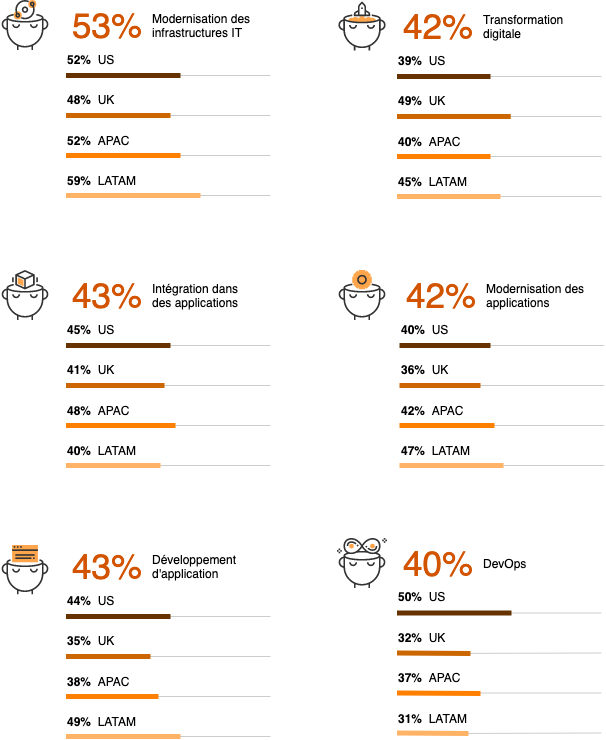
\includegraphics[scale=0.65]{./img/Use_os.png}
						\caption{Secteur d'application de l'open source}					
					\end{figure}
					\clearpage

				\paragraph{Les domaines informatique de l'open source dans l'entreprise\\}

					Ce relevé indique pour quels domaines métier de l'informatique nous utilisons majoritairement l'open source:

					\begin{figure}[h]
						\center
						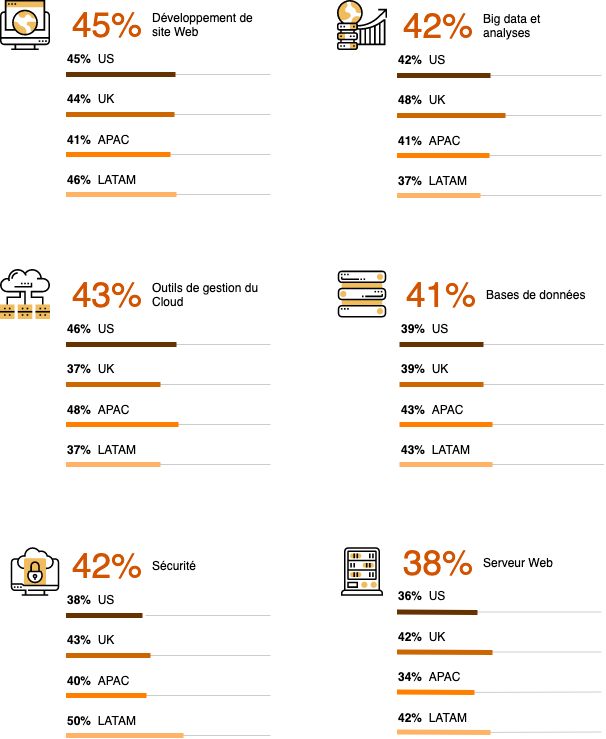
\includegraphics[scale=0.65]{./img/Domain_os.png}
						\caption{Domaine d'application de l'open source dans l'IT}					
					\end{figure}
					\clearpage


				\paragraph{Les réticences encores présente sur l'open source\\}

					Malgré l'impact bénéfique de l'open source pour les entreprises, il reste encore quelques inquiétudes planant au dessus de l'open source et des réticence à son utilisation généralisée.

					A travers le hack et le piratage de produit open source, les entreprise positionnent la sécurité de l'open source comme une inquiétude majeure.

					\begin{figure}[h]
						\center
						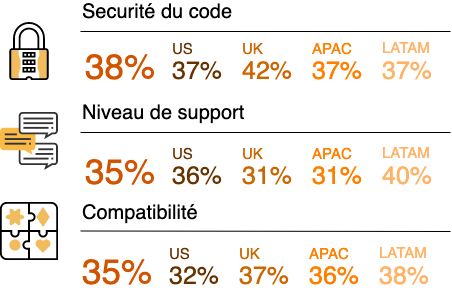
\includegraphics[scale=0.75]{./img/Barreer_os.png}
						\caption{Causes principales des réticences à l'open source}					
					\end{figure}
					\clearpage

				\paragraph{L'évolution de l'utilisation de l'open source\\}

					Beaucoup d'entreprises continuent tout de même à utiliser des logiciels propriétaires, mais cette tendance tend à diminuer sur les 2 prochaines années. Ceci grâce aux nouvelles technologies provenant du \gls{web 3.0}, notemment la \gls{conteneurisation}, qui est considéré comme un brassage de produit collaboratif open sources.De nombreuses entreprise aujourd'hui se tourne vers des solutions de conteneurisation, due à l'open source.
					
					\begin{figure}[h]
						\center
						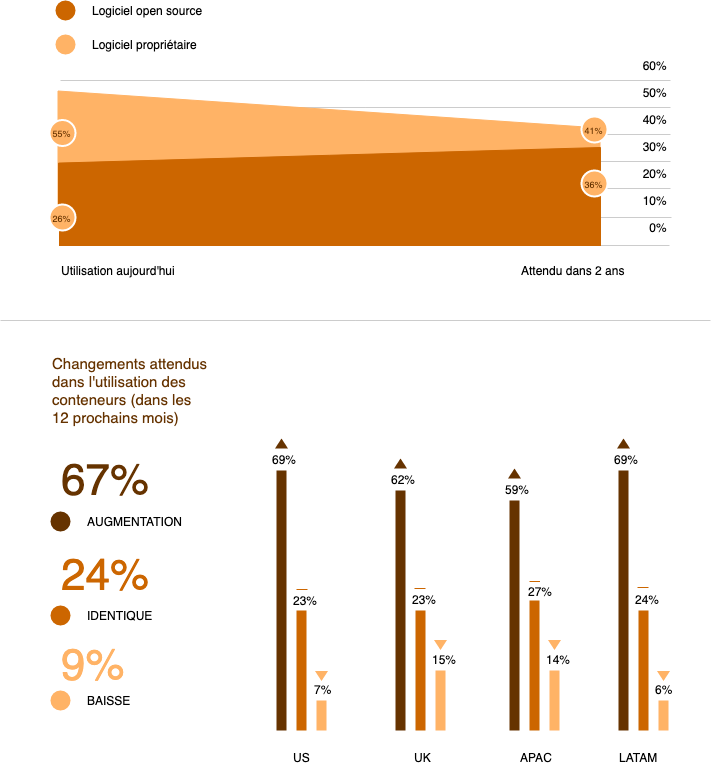
\includegraphics[scale=0.65]{./img/Enterprise_os.png}
						\caption{Évolution de l'open source dans les années à suivre}					
					\end{figure}
					\clearpage
					

		\subsection{Les éditeurs open source}

			\subsubsection{Zoom sur l'éditeur}

				L'éditeur, c'est celui qui détient les droits du produit, en assure le développement, la promotion, la diffusion et le support.\\
			
				La seule différence avec l'éditeur de logiciels pour l'éditeur open source est qu'il publie son produit sous licence open source. Sinon l'investissement dans le développement du produit et son marketing est le même qu'un produit propriétaire.
				Ce modèle a été élu pour permettre de briser les position acquise d'oligopoles sur le marché du logiciel.
				Il s'agit donc majoritairement de petites entreprises éditrice qui font du support et du développement du produit leur credos.
				Développer un programme open source coute (un peu) moins cher pour ces entreprises car :

				\begin{enumerate}[font=\color{burntorange}]
		 			\item Elles peuvent s'appuyer sur autant de brique que la licence de son logiciel lui permette.
		 			\item Elles bénéficient de contributions communautaire, que je détaille ultérieurement.
			 		\item Elles possèdent généralement plus de développeur passionné participent à son travail.
				\end{enumerate}

				Nous parlerons plus en détail du modèle économique des éditeurs dans la partie sur le marché de l'open source.
				Généralement, l'éditeur fait le choix de partir sur une licence GPL car elle présente pour eux deux avantages considérables:


				\begin{enumerate}[font=\color{burntorange}]
		 			\item Du fait de sa popularité, elle est parfaitement lisible et compréhensible ce qui la rend gage de tranparence.
		 			\item Elle empêche les autres de se faire de l'argent sur son dos car elle interdit l'intégration du produit dans un développement propriétaire.
				\end{enumerate}

			\subsubsection{L'aspect communautaire}

				L'éditeur open source a à sa disposition une communauté qui pourra l'aider non seulement dans le support sur les ressources open source qu'il utilise mais également au développement et au support de son oeuvre.

				Au sein de la communauté il est possible de distinguer deux types d'acteurs:

				\begin{description}[font=\color{burntorange}]
					\item[les développeurs indépendants: ] Qu'il s'agisse de gloire, de monté en compétence sur un domaine ou d'altruisme, il existe des développeurs qui soutiennent le développement de produit et participent au support.
					\item[Les contributeurs et entreprises contributrices: ] Certaines entreprises favorisent l'aide et autorise leurs employés à travailler une partie de leurs temps d'activité sur des projets open sources.
				\end{description}

				Parmis ces contributeurs, on retrouve beaucoup de salariés d'entreprise IT et ce pour plusieurs raisons comme:

				\begin{itemize}[label=\textbullet, font=\LARGE \color{burntorange}]
					\item Le marketing: statuer que l'on a un développeur qui travaille sur un « Grand projet » pour dorer son image et promouvoir son entreprise.
					\item La gouvernance: car cela permet d'avoir son mot à dire sur les orientations stratégiques d'un produit
					\item Le socle technique: Plus il y a de contributions à un socle de produit open source dont l'entreprise est utilisatrice, meilleur sera leur business.
					\item La maitrise du produit: Monter en compétence et proposer du support sur ce produit.
				\end{itemize}

				\paragraph{Les contributions communautaires\\}

				%A retravailler
				Les éditeurs open source comptent en général assez peu sur les apports communautaires, du moins sur le coeur de leur produit. Ils les acceptent car c'est dans la logique de l'open source, mais ne les encouragent guère et l'on peut penser qu'il ne leur déplait pas de garder la maîtrise de leur produit.\\

				A noter que si son morceau de code est accepté, le contributeur devra généralement signer un accord spécifique qui permet à l'éditeur de disposer librement de son code. C'est assez naturel, car si chaque contributeur pouvait spécifier ses propres conditions de licence, le produit final serait un enchevêtrement de licences indémêlables.\\

				Afin de bénéficier d'une dynamique communautaire, tout en conservant la maîtrise du noyau de leur produit, certains éditeurs mettent en place un dispositif d'extensions, qui permet d'apporter des enrichissements au produit, de manière propre et indépendante du noyau, en assurant la compatibilité avec les versions futures.

				\paragraph{Le noyau et les extensions, un écosystème\\}

				Le modèle qui semble le plus efficace, et le meilleur compromis, est celui qui distingue le noyau du produit, sous la responsabilité de l'éditeur, et les extensions, réalisées par la communauté.

				Les principes de séparation sont les suivants:

				\begin{itemize}[label=\textbullet, font=\LARGE \color{burntorange}]
					\item Le noyau doit être d'une grande robustesse, il est certifié par l'éditeur, les contributions externes y sont rares
					\item L'inferface entre le noyau et les extensions est bien documentée et stabke, c'est à dire qu'un changement de version du noyau n'implique pas, du moins le plus souvent, un changement de version des extensions.	
					\item L'éditeur stimule la réalisation d'extensions, car elles donnent de la valeur à son produit et témoignent aussi de l'existence d'une communauté, en soi un gage de pérennité. L'éditeur offre en général une plateforme de mise à disposition de 
				\end{itemize}

				Ce modèle noyau/extensions est celui qui réalise le meilleur point d'équilibre entre les rôles respectifs de l'éditeur et de la communauté, réunissant la garantie et l'engagement de l'éditeur avec le dynamisme et l'énorme capacité de développement de la communauté.

			\subsubsection{Les supports de l'open source}

				% A retravailler
				Le support dans le monde du logiciel, c'est la capacité à apporter de l'aide dans l'utilisation du programme et à corriger le programme le cas échéant.\\
				
				Le support peut s'adresser aux utilisateurs finaux, comme aux exploitants du programme, ou encore aux programmeurs travaillant sur le programme.\\
				
				Le déploiement de programmes pour des tâches critiques, en particulier dans des entreprises, requiert absolument un support, car le risque d'une situation de blocage est trop important, cela que ce blocage soit dû à une anomalie ou à un mauvais usage, mauvaise configuration, incompatibilité, etc.

				\paragraph{Le support de l'éditeur\\}

				Du côté des éditeurs open source (MySql, eZ Publish, OpenERP, ...), la question est différente: l'éditeur est une société commerciale et son business model est essentiellement basé sur son offre de support. Ici donc, le dispositif de support est très proche de celui des produits propriétaires. Pas identique toutefois car \textit{en parallèle, en complément} au support payant de l'éditeur, il existe souvent un support communautaire, plus ou moins vivace selon les produits.Mais le plus souvent, les corrections touchant au code ne sont assurées que par l'éditeur.\\

				Pour les nouveaux éditeurs de l'open source commercial, le support produit est le fondement du business model, il est leur raison de vivre, leur unique source de revenus. On peut donc s'attendre à un support de grande qualité.

				\paragraph{Le support de la communauté\\}

				Les produits communautaires bénéficient avant tout d'un support communautaire. C'est à dire basé sur le volontariat de développeurs impliqués, qui répondent aux questions des utilisateurs sur les mailing-lists et forums. Et basé également sur le suivi et la prise en charge des anomalies sur les plateformes de développement communautaires.\\

				Lorsque la communauté est active, comme c'est le cas autour des grands produits, ce support communautaire peut être d'une très grande efficacité, d'une très grande réactivité, très supérieur à un support commercial.\\

				Nous verrons plus tard comment améliorer cette gestion de la communauté dans la partie optimisation des ressources.

		\subsection{Le consommateur}

			\subsubsection{Qui est le consommateur ?}

			Je classifie les consommateurs en trois catégories distinctes :
			\begin{description}[font=\color{burntorange}]
				\item[Les end-users:] Ce sont les clients finaux du produit open source. Si le logiciel open source à pour vocation d'être utilisé comme tel par le grand public ou bien parmis les entreprises, on considère ces personnes comme des utilisateurs finaux ou \textit{« end-users »}. Ils utilisent le logiciel, remontent leurs besoins d'amélioration, de correctifs et de support.
				\item[Les contributeurs et la communauté:] consomme l'open source car ils y contribuent, en adaptant certains besoins du logiciel par la création d'extension, par l'aide au développement, et tout soutient qui implique l'utilisation du produit de l'éditeur.
				\item[Les autres éditeurs et prestataires:] Comme nous l'avons aperçu précedemment, une licence open source permet de bénéficier de toutes les ressources sous la même licence. Les développeurs chez les éditeurs et prestataires réalisent des aggrégats de différentes solutions open sources à laquelle ils intégrent la leur. Nous le verrons plus en détail dans la partie concernant l'intégration de solution.
			\end{description}

			Il est important de considérer que nous somme tous des consommateurs appartenants à la catégorie « end-user » car aujourd'hui, nous avons tous utilisé au moins une application, une partie de logiciel qui utilise de l'open source. Même sans en avoir conscience.\\

			Favoriser l'open source pour ces consommateurs c'est leur permettre une expérience plus libre dans leurs besoins. Voyons à présent quels en sont leur bénéfices.
			
			\subsubsection{Les bénéfices de l'open source pour le client}
			%A retravailler

			Bien sûr, les bénéfices économiques sont parmi les premières raisons dans le choix de solutions open source. Même si « libre ne signifie pas gratuit », ces solutions ont toujours un coût de possession sensiblement moins élevé que leurs équivalents propriétaires.\\

			D'autant que les prix de prestations tendent aussi à être moins élevés, car l'ouverture du produit facilite la diffusion de la connaissance.\\

			Mais au fur et à mesure que ces solutions arrivent à maturité, le moindre coût n'est plus le premier critère de choix.\\
			Les principaux arguments sont alors :\\


			\begin{itemize}[label=\textbullet, font=\LARGE \color{burntorange}]
				\item \textbf{La non-dépendance}, ou moindre dépendance, par rapport à un éditeur. On sait que changer d'outil peut coûter très cher, et les éditeurs peuvent être tentés de profiter de la vache à lait que constituent ces clients devenus captifs. En anglais, on parle de vendor lock-in, le verrouillage par le fournisseur.
				\item \textbf{L'ouverture} est également un argument de poids. Les solutions open source sont en général plus respectueuses des standards, et plus ouvertes vers l'ajout de modules d'extension.
				\item \textbf{La pérennité} est un autre critère de choix fort, nous y revenons plus loin.
				\item \textbf{Et la qualité} finalement, car dans beaucoup de domaines les solutions open source sont réellement, objectivement, supérieures. Le très grand nombre de déploiements et donc de retours d'expérience, mais aussi leur modèle de développement et leur intégration de composants de haut niveau, permet à beaucoup de surclasser les produits propriétaires souvent vieillissants.
			\end{itemize}

			A quoi on peut ajouter le plaisir, pour les informaticiens, d'utiliser des programmes dont ils peuvent acquérir une totale maîtrise, sans barrière ni technique ni juridique.

		\subsection{Où trouver de l'open source ?} 

			Que l'on souhaite démarrer son projet open source ou contribuer au patrimoine du Logiciel Libre, de nombreuses plateforme et espace web permettent le stockage et la redistribution de ces projet open sources.

				\begin{figure}[h]
					\center
					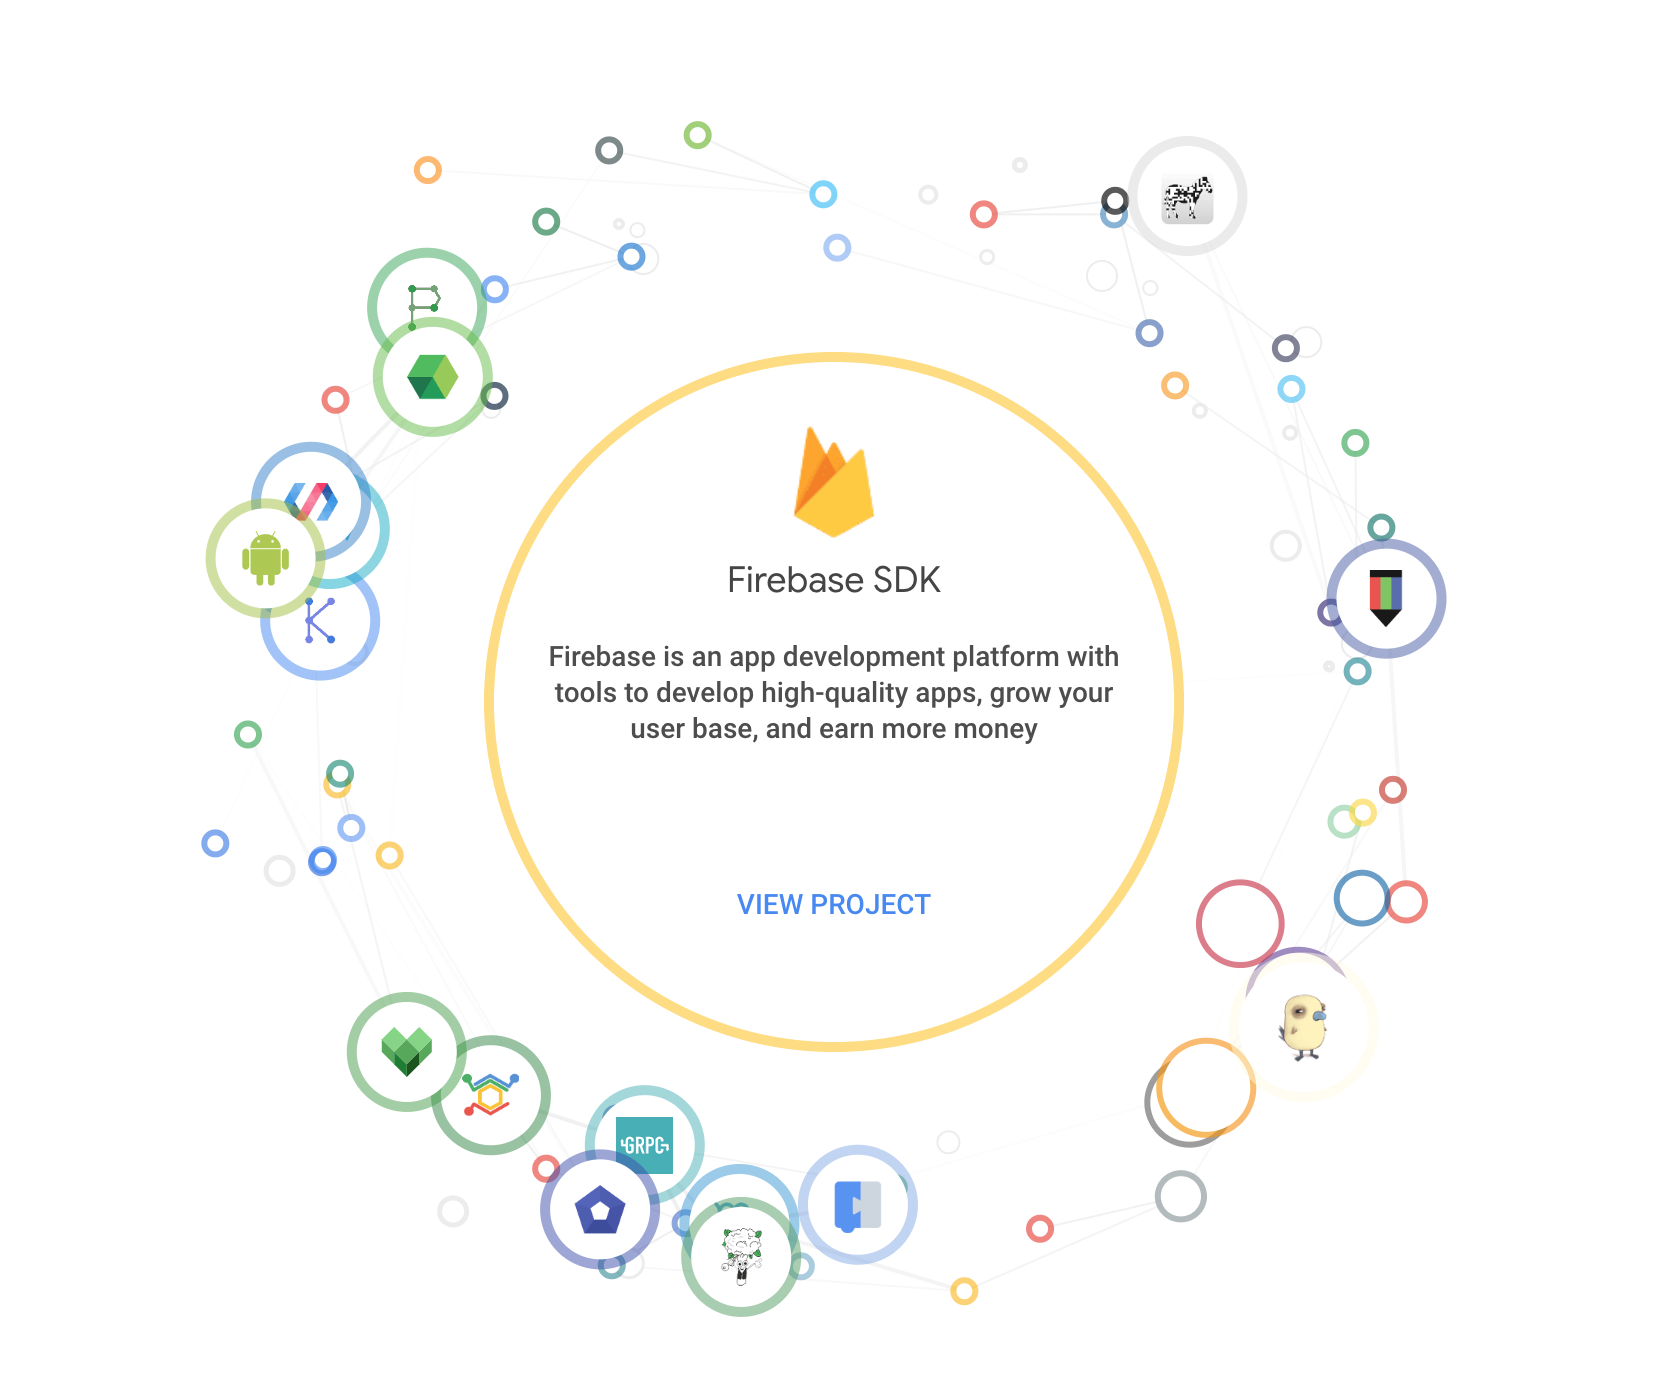
\includegraphics[scale=0.40]{./img/google_os}
					\caption{Interface de google open source}					
				\end{figure}


			\paragraph{Plateforme de dépot de code}
				% A retravailler

				\subparagraph{Github\\}
				La plateforme «open source» par excellence centralisant le code source des plus grandes entreprises du monde: Microsoft, Netflix, Facebook entre autres.
			
				\subparagraph{Bitbucket\\}
				Très similaire à GitHub, Bitbucket est un hébergeur de code source libre qui permet à chacun de s’intéresser à des solutions libres.

			\paragraph{Plateforme de promotion de projet}

				\subparagraph{Google Open Source\\}

				Avec plus de 2000 projets libres sous sa tutelle, Google Open Source est un incubateur des nouveaux projets libres sur le marché.
				La plateforme est simple, rechercher un projet comme une recherche google, ou attendre la présentation de différents projets et laisser la magie opérer 

				\subparagraph{Github Explore\\}
				L'interface prévue pour trouver un projet open source auquel contribuer et offerte par la plateforme de dépot Github.

				\subparagraph{Open source friday\\}
				Github propose comme date de rendez-vous tout les vendredi pour contribuer chaque semaine à enrichir le logiciel libre pour les curieux et les plus passionnés.

				\subparagraph{24 pull request\\}

				Chaque année pour la période de Noël, 24 Pull Request organise un moment de développement logiciel sur de l'open source avec comme objectif de remercier les éditeurs et leurs projets qui nous aident tant.
				En 2018, 1364 contributeurs ont participés sur 3321 différents projets open sources.

				\subparagraph{Code triage\\}

				La plateforme CodeTriage est non seulement utile pour trouver son projet et démarrer rapidement dessus mais nous envois également un mail quotidien pour nous soutenir et nous rappeler nos engagements.

				\subparagraph{Contributor ninja\\}

				Ici plus qu'un évenement c'est une plateforme avec une interface rapide, pour contribuer très rapidement (tel un ninja!) à n'importe quel projets selon le langage de prédilection du contributeur potentiel.

				\subparagraph{Up for grabs}

				Pour vaincre toute forme de procrastination et la peur de faire le premier pas (qui handicape si souvent l'homme), up for grabs permet de rapidement trouver la bonne chaussure à son pied et se lancer dans la contribution à l'open source. Le processus est simple :

				\begin{itemize}[label=\textbullet, font=\LARGE \color{burntorange}]
					\item Lire les quelques ligne du guide de contribution
					\item Installer le projet localement
					\item Laisser un message sur la tâche que l'on s'apprête à faire
					\item Se lançer dans le travail !
				\end{itemize}

				\subparagraph{First Timers Only}

				On peut être pris au dépourvu lorsque l'on s'aperçoit que l'open source est un monde bien vaste que l'on ignorait. Pour celà, First Timers Only nous donne les clés pour débuter l'aventure dans l'open source en tant que contributeur.


			\paragraph{Association du libre\\}

				\subparagraph{Capitole du libre}
				Association française du code source libre que j’ai eu le plaisir de rencontrer à l’ENSEEIHT, leur chaîne youtube fournit des présentations utiles à ce sujet.

				\subparagraph{April}
				Une association française qui contribue à l’open source via des campagnes et thèmes de travail autour du sujet.
		
		\paragraph{Pour conclure\\}

			L’open source est donc un mouvement important. Il apporte des valeurs de liberté, solidarité mais aussi des bénéfices tant pour les citoyens que pour les entreprises. 
		
	% --------------------------------------------------%
	%     												%
	%             Optimisation des ressources			%
	%       										    %
	% --------------------------------------------------%
	\section{Optimisation des ressources} % in progress % Utiliser des livres sur comment monter et créer son logiciels open source et mettre en concordance led élement apporté dans Reflechissez et devenez riche + Oser la confiance

		\paragraph{Concept de l'optimisation\\}

	 		Le succès d'un projet open source dépend pour beaucoup de leur code, mais pas uniquement. De leur concept, de leur capacité à faire connaître votre projet, à faire naître une communauté, à piloter une startup aussi, et le cas échéant à convertir leur succès en revenus, qui pourront assurer la pérennité de leur aventure.

		\subsection{Rendre le libre populaire}

			\subsubsection{Pareto revisité}
			Une étude sur la participation de développeur et le code total rédigé rapporte que si l'on prend un projet ou 200 programmeurs participent, seulement, 10 d'entre eux ont écris 50\% du code.

			\subsubsection{L'enseignement du logiciel libre}

			Comme mentionné dans l'introduction de ce document, le logiciel libre me semble pas suffisemment enseigné. 

			\textbf{Qu'est-ce que j'entend par enseigner le logiciel libre ?}

			\paragraph{Susciter l'intérer du libre\\}

			Enseigner un logiciel libre par la mise en place d'efforts spécifiques à celui-ci. Ce n'est pas en utilisant sans le savoir de l'open source ou en cherchant spécifiquement à remplacer tout logiciel propriétaire par du libre que l'on enseigne l'open source. Il est nécessaire d'expliquer les mécanismes liés à l'open source, de prendre le temps d'informer sur toute l'importance et ce qui gravite autour de l'open source.\\
			Ceci afin de permettre à des centaines de programmeur éparpillé sur la planète à coopérer de façon cohérente sur la réalisation des millions de lignes de code.\\

			Celà passe également par la mise en relation des étudiants avec les communautés de développeur.

			\paragraph{Améliorer la recherche sur l'open source\\}

			Il est nécessaire d'encourager la recherche qui se développe autour des logiciels libre et fournir des outils nouveaux pour accompagner leur essor.\\

			Les plateformes distribuant l'open source sont à première vue trop réservée à la communauté de développeurs, des « Nerds » qui développent la nuit .

			\paragraph{Un gisement d'emplois futur\\}

			Tant par ses valeurs humanistes que par la contribution au patrimoine de l'humanité, l'open source doit être vue comme un bien commun qu'il faut cultiver en commun.\\

			Tout autant que l'art qui est exposé dans de nombreux musée que l'on rends accecibles les 1er dimanche du mois gratuitement pour contribuer à la culture de l'homme, l'open source devrait être considéré de même.\\

			Au coeur de l'activité industrielle encore méconnu, l'open source c'est \textbf{4,46 Md d' \euro{}} de \acrshort{ca} en 2017. \textbf{4000 emplois} nets ont été estimée d'ici 2020. La France est le leader Européen de l'open source. Et pourtant, le système éducatif actuel ne perçoit pas ce gisement. 

		\subsection{Intêret et communauté}

		\subsection{Le modèle noyau extension}

			Comme précedemment évoqué, il s'agit ici du meilleur schéma de développement connu pour déployer son activité open source. Il s'agit d'identifier et d'offrir noyau logiciel et mettre en place des points d'attaches pour les différentes extensions que l'on souhaiterai apporter.

			On dénote plusieurs avantages à ce modèle d'architecture:

			\begin{itemize}[label=\textbullet, font=\LARGE \color{burntorange}]
			\item Ne pas faire grossir inutilement un programme en se concentrant sur l'essentiel du business et de sa fonctionnalité.
			\item Jouer sur l'aspect modulable et simple du logiciel et concurrencer les logiciels propriétaires qui, sous pressions, rajoutent de plus en plus de fonctionnalités sur leur logiciel jusqu'à le rendre trop lourd .
			\item Déjouer la concurrence sur le marché, car la communauté se concentre sur la création et l' amélioration perpetuelle des extensions. Donnant un coup de neuf tout les jours.
			\item Eviter de destabiliser son logiciel car les fonctionnalités peuvent être ajouté sous forme de modules.
			\end{itemize}

			Le modèle noyaux-extension permet de tracer cette frontière entre l'éditeur et la communauté tout en s'assurant que la communauté trouve sa place au sein du produit et que chacun puisse répondre à son besoin.

			Pour favoriser la mise en place et le maintient du modèle noyau-extension, l'éditeur met généralement en place une plateforme pour accueillir ces extensions afin d'avoir une meilleur visibilité, classer par popularité, trier selon les besoins et de rendre gloire aux auteurs de ces extensions.
			
		\subsection{Eveiller sa communauté}

			Afin de faire naitre et grandir sa propre communauté autour de son produit open source, il existe déjà quelques points clés ou « best practices » dont il est bon de rappeler:

			\begin{itemize}[label=\textbullet, font=\LARGE \color{burntorange}]
				\item \textbf{Semer la graine} en mettant en ligne son code source. Être patient vis à vis de l'épanouissement de la communauté qui va prendre racine. Celà ne prendra pas quelques jours mais est un travail de longue halaine.
				\item Être \textbf{transparent} tant dans son projet et ses orientation que dans la \textbf{gouvernance} du projet.
				\item Choisir et \textbf{décréter son support d'échange} avec la communauté. Afin de centraliser la communauté sur ses outils.
				\item Instaurer sa \textbf{politique de l'open source} en proposant un modèle \textbf{noyau-extension}, celui qui fonctionne pour le mieux. Bien préciser quels sont les aspects que l'on veut retrouver dans notre \textbf{vision} open source.
				\item \textbf{Inspirer des valeurs}: le logiciel que l'on va construire n'a pas de but lucratif ou du moins il est moindre.Ceci aide à construire la communauté plus facilement car elle n'aura pas l'idée qu'on génère de l'argent sur son dos. On aspire à aider, changer le monde. Il faudra trouver l'idée d'\textbf{une mission} que les gens adoptent.
			\end{itemize}

	% --------------------------------------------------%
	%     												%
	%              Etude du consommateur				%
	%       										    %
	% --------------------------------------------------%
	\section{Etude du consommateur} % in progress

		\subsection{Les entreprises adoptent l'open source}

			L'open source croît sans cesse et il n'est plus une en,treprise dont une part du système d'information ne soit construit avec des composants et solutions open source. L'open source et partout on retrouve l'expression anglo-saxonne « Open source is going mainstream», l'open source est devenu un standard, une normalité.\\
			%A retravailler

			Pour une grande majoritée de clients, de DSI, quelle que soit la taille d'entreprise ou son scteur d'activité, les solution Open source sont désormais pleinement acceptées, et leur bénéfices parfaitement appréciés. C'est énorme. La banalisation ici, est bien une forme de consécration. Chez les prestataires, ce marché à attiré du monde notemment avec les \acrshort{ssii}.\\

			Le catalogue de service lié à l'open source s'aggrandit chaque jour et aide à convaincre les DSI les plus exigentes.

	% --------------------------------------------------%
	%     												%
	%            Le marché de l'open source			    %
	%       										    %
	% --------------------------------------------------%

	\section{Le marché de l'open source} % in progress

		\paragraph{Libre n'est pas gratuit \\} 

			C'est bien l'un des principes de l'open source. Même si l'on y a pour vocation de s'étendre et de distribuer son produit, il est nécessaire, si ce n'est vital pour certains éditeurs de trouver une source de revenus pour leur logiciel.\\
			Il faut savoir qu'il existe une différence entre faire payer un logiciel propriétaire et un logiciel open source. 
			\begin{description}[font=\color{burntorange}]
				\item [Payer un logiciel propriétaire: ] permet non seulement d'apporter des revenus à une entreprise mais d'obtenir un « droit de possession », d'acquisition du logiciel.
				\item [Payer un logiciel open source: ] N'est pas un prix d'acquisition ni un droit d'utilisation mais une source de revenus à l'éditeur pour permettre au logiciel de prospérer.
			\end{description}

		\subsection{Les acteurs de l'open source}
			Il existe dans l'open source 4 grands acteurs:

			\begin{description}[font=\color{burntorange}]
				\item[Les fondations:] telles que Apache ou Eclipse, sont des organismes à but non lucratif qui stimulent et pilotent le développment de grands produits open source.
				\item[Les distributeurs:] Redhat, Canonical (Ubuntu) ou Mandriva sont des distributeurs (très souvent éditeurs par la même occasion). Ils sélectionnent des outils et composants autour d'un noyau Linux, en assurent le packaging, la distribution et le support
				\item[Les éditeurs:] Diffusent des logiciels sous licence open source, ils réalisent la promotion de leurs produits et proposent du support
				\item[Les prestataires: ] Ils vendent des services sur l'open source. Il peut s'agir de conseil, d'intégration, de support, de la formation, des solutions d'hébergement, etc.
			\end{description}

			Je m'intéresse particulièrement aux éditeurs et aux prestataires de l'open source qui devront mettre en place des solutions pérénisant financièrement leur activité.\\

			Et de la prospérité les éditeurs en ont bien besoin car pour les autres acteurs, la taille, la mission et le produit présenté ne pose plus aucune difficulté de revenu. Doit-on encore se soucier du bon développement de Linux et de sa communauté ? Ces géants de l'open source, association à but non lucratif, ont des moyens marketings (plus de 60\% de leur revenus) et financier bien supérieurs aux éditeurs et prestataires qui restent pour la majorité des petites et moyennes entreprises.

			\textbf{Comment fonctionne donc le modèle économique ou « business model » de ces entreprises ?}\\

		\subsection{Chez les éditeurs}

			Même s'ils bénéficient de l'open source pour réduire leur coût de ressources, celle-ci ne comblent pas les besoins de financement de la partie développement en interne, hébergement, marketing. Il est donc nécessaire de trouver des sources de revenus pour les éditeurs.

			Parmis celles-ci, on distingue 3 principales sources pour l'éditeur:

			\begin{itemize}[label=\textbullet, font=\LARGE \color{burntorange}]
				\item Vendre des licences
				\item Vendre du support
				\item Vendre de l'intégration
				\item Autres sources de revenus
			\end{itemize}

			\subsubsection{Vendre des licences}

			Même s'il est interdit de faire payer l'utilisation d'un logiciel open source, les éditeurs ont bien compris commment faire bon usage de la « double licence ».

			\paragraph{Double licence commerciale\\}

			Il est possible de distribuer une oeuvre dérivée utilisant le programme sans diffuser ses sources à l'aide d'une licence commerciale.\\
			Le programme officiel open source est gratuit mais sa version dérivée elle est payante à travers l'achat de licence commerciale.\\

			Pour l'entreprise MySql, la vente de licence représente plus de la moitié du \acrfull{ca}. Pour d'autre, ce n'est pas une source de revenu suffisante car leur finalité est de faire un \textit{site} et non \textit{un produit}.

			\paragraph{Les extension payantes\\}

			L'éditeur peut proposer des extensions aux fonctionnalités présente dans le logiciel open source. Le logiciel initial est suffisemment de qualité et donne envie de payer quelques extension \textit{optionnelles} supplémentaire pour le confort et le besoin de l'utilisateur.

			\paragraph{Un support uniquement sur licence commerciale\\}

			Ici aussi, le logiciel est sous licence open source mais si l'on désire avoir le moindre support dessus, il faudra se tourner vers son confrère et sa licence commerciale.

			\subsubsection{Vendre du support}

			La prestation de support est une source principale de revenu pour l'éditeur, même s'il doit pour celà faire face à la concurrence potentielle de prestataires tiers que je précise juste après.

			Le support d'un logiciel inclut généralement :

			\begin{itemize}[label=\textbullet, font=\LARGE \color{burntorange}]
				\item L'accès privilégié aux correctif et ressources spécifique
				\item Une prise en chage des problèmes (anomalies, utilisation, mise en oeuvre ...)
				\item Des prestation d'audit, de certification, ou de prise de contrôle à distance, ainsi que la surveillance proactive et les corrections.
			\end{itemize}

			On peux distinguer différent modèles de financement concernant la vente de support:

			\paragraph{Uniquement le support\\}

			Certains éditeurs misent uniquement sur la vente de support. Le logiciel est gratuit mais le support lui est payant. Ce modèle de financement fonctionne pour certaines entreprises comme Tiny(OpenERP), Nuxeo.\\

			Le problème est qu'en cas ou le support n'a pas été utile l'année souscrite pour cause de stabilité du logiciel, le client voudra surement le résilier pour la suite.\\

			Plus le produit est de qualité, moins le support est facile à vendre car le client rencontre moins de difficultés.\\

			L'avantage est que plus on avance dans la technologie et plus la concurrence est présente on doit donc sortir des nouveautés constemment ce qui fragilise le produit et le rend instable.Le support est donc précieux dans le cadre professionnel.

			\paragraph{Faire payer la stabilité\\}

			Pour d'autre éditeurs, la stabilité d'un logiciel peut devenir source de profit. L'idée est de proposer deux logiciel:\\

			\begin{itemize}[label=\textbullet, font=\LARGE \color{burntorange}]
				\item Celui en licence open source sera classifié de « community edition ». Il sera présenté comme instable, pas entièrement testé, à ne pas déployer en production
				\item Tandis que le logiciel sous licence non-libre sera la licence sécurisée, une version « enterprise-ready », « fully tested ».
			\end{itemize} 

			Au final, la version community, c'est celle en cours de développement donc en avance de phase alors que la version entreprise c'est celle qui a été \textit{gelée} dans un état dit \textit{« stable »}.\\

			L'éditeur peut alors diffuser et promouvoir son produit à travers la version community, et apâter les entreprises dans la version payante ou généralement le support est packagé avec.\\

			L'éditeur jongle sur la stabilité de la version community en la rendant suffisamment stable pour donner envie de l'utiliser mais inciter fortement les entreprises à prendre la version sous licence commerciale qui sera accompagnée du support.

			\paragraph{Fonctionnalités avancées\\}

			Pour l'éditeur, un autre business model et celui de la fonctionnalitée avancée.\\
			La version community et enterprise n'est pas différente d'un point de vue stabilité mais ce sont les fonctionnalitées présente qui sont réduites sur la version community.\\

			Ceci permet de se dégager du paradigme « libre = instable » totalement infondé.\\

			La difficulté pour l'éditeur va être d'avoir suffisemment de fonctionnalitées pour rendre la version libre intéressante mais d'avoir une forte valeur ajoutée sur les fonctionnalités dans la version payante.

			\subsubsection{Vendre de l'intégration}

			Pour les éditeurs qui ne sont pas mondialement connu, il est possible de trouver la rentabilité en proposant l'intégration de son produit open source. C'est un moyen de démarrer dans le milieu sans trop de risque mais qui n'est pas « \gls{scalable} ». On ne peux s'étendre à l'étranger si l'on est le concurrent direct de ses intégrateurs partenaires. On reste donc sur un marché réduit.

			\subsubsection{Autres sources de revenus}

			\paragraph{Les campagnes de crowdfunding\\}

				En Mai 2019, la plateforme d'hébergement de logiciel Github, que nous détaillerons plus tard, propose un programme de sponsoring et de crowdfunding.

			\paragraph{Vendre des extensions\\}

				Selon le modèle noyau-extension, nombre d'éditeur open source on trouvé leur part de marché dans la vente des extensions. Bien que réalisées généralement par la communauté, l'éditeur peut considérer la vente des extensions réalisées afin de rémunérer les contributeurs mais prélève un montant sur la vente d'extensions. De cette manière, l'éditeur de la solution open source Magento pour le e-commerce, prélève 30\% du prix de vente des extensions à la manière de l'Apple Store.
			
		\subsection{Chez les prestataires}

			Pour les prestataires de l'open source, le business model est basé sur la vente de prestation et d'expertise sur les produit.

				\paragraph{La naissance des \acrfull{ssll}\\}

				L'une des activité du prestataire est la gestion du support de solution open source. Il existe une telle diversité de composant open source qu'il est difficile pour un prestataire unique de se concentrer sur le support dudit logiciel.\\

				Dans certains cas, la prestation est demandé par l'éditeur. Dans d'autre, c'est un prestataire tiers qui assurera du support, sans doute moins légitime et moins expert que l'éditeur lui-même mais aussi moins chère.\\

				Ainsi est né en France le concept de \acrshort{ssll}, une société qui propose d'assurer le déploiement et le support de configuration multi-produits à base d'open source.\\

				Un peu plus tard les \acrfull{ssii} généralistes prennent partis en ouvrant des centre de support open source.

				\paragraph{Intégrer des solutions open sources\\}

				Le principe de ce modèle est de construire une application globale, un système d'information, en assemblant des logiciels open sources.\\

				Il faudra donc également assurer le support de ces créations.\\
				La valeur ajoutée ici est dans le choix des solutions à intégrer. 

				Il y a tellement de possibilité de solution dans l'open source qu'il est nécessaire d'étudier correctement le marché en fesant les bons choix. Ceci passe par une action de veille permanente sur les solutions disponible, afin de déceler les opportunité et produits prometteur pour avoir la création la plus solide et pérenne possible.

		\subsection{Communication par ses atouts}

			En guise de communication, l'open source n'a pas tant besoin de budget marketing. En effet il puise sa force là ou il a pris racine, c'eest à dire dans sa communauté. Nul besoin de mettre de faux posts et avis sur touts les blogs du net, la vérité et la promotion de l'open source se fait principalement par la communauté.

			Le caractère open source permet en général de diffuser bien plus rapidement son produit.

			La communauté utilise donc tout support moderne de communication pour diffuser, twitter, poster ces informations

			Ainsi malgré le marketing ordinaire (campagne publicitaires, affiches, buzz-marketing ...) que ne peuvent se permettrent bon nombre d'éditeur, ils peuvent espérer que le marketing moderne 2.0, qui est la force et le fondement de l'open source, prenne la relève.











